\subsection{Porównywanie zapytań}
W rozdziale zostanie przedstawione działanie polecenia EXPLAIN. Polecenie to umożliwia uzyskanie informacji o planie wykonania zapytania. Jest podstawowym sposobem określenia, w jaki sposób MySQL wykonuje zapytania. Analiza wyników EXPLAIN jest zdecydowanie bardziej użyteczna od mierzenia czasów zapytań. Na czas wykonania zapytania może mieć wpływ kilka czynników, które wprowadzą nas w błąd podczas badania wydajności danego zapytania. Pierwszym z nich jest cache zapytań. Przeprowadzając testy zapytania przy włączonym buforze zapytań, może zdarzyć się, że rezultat zapytania zostanie zwrócony z tego właśnie bufora. Doprowadzi to do sytuacji, kiedy nawet najbardziej niewydajne zapytania będą zwracane w ułamki sekund.  Problem ze zwracaniem wyników z bufora zapytań możemy rozwiązać poprzez wyłączenie bufora zapytań lub dodanie modyfikatora SQL\textunderscore NO\textunderscore CACHE do zapytań. Drugim czynnikiem zaburzającym mierzenie czasów wykonania zapytań jest bufor MySQL. MySQL stara się przechowywać w pamięci często używane dane, dla przykładu indeksy. Jeżeli wykonujemy zapytanie dla tabeli, której indeks nie znajduje się w pamięci. Serwer pobiera indeks z dysku, co trwa. Następnie poprawiamy zapytanie w celu poprawienia wydajności i wykonujemy, aby sprawdzić, czy nasze działanie poprawiło wydajność. Tym razem cały indeks znajduje się w pamięci i zapytanie wykonuje się wielokrotnie szybciej. Mierząc jedynie czasy wykonania obu zapytań, możemy dojść do fałszywego wniosku, że drugie zapytanie jest zdecydowanie bardziej wydajne, nawet jeżeli w rzeczywistości nasze działanie doprowadziło do pogorszenia wydajności zapytania. W takim przypadku dobrym rozwiązaniem wydaje się kilkukrotne mierzenie czasów, obliczenie średniej i na tej podstawie porównywanie wyników. Dodatkowo nasz serwer rzadko kiedy jest całkowicie odcięty od świata. Bardzo często będziemy testować wydajność zapytań na tabelach, które są w równocześnie modyfikowane w tle. Dla przykładu jeżeli testujemy zapytanie na tabeli, na której wykonywane są w tym momencie operacje zapisu, nasze wyniki będą zwracane w czasach, które będzie nam bardzo trudno interpretować. Dodatkowo na czasy wykonywania zapytań wpływ może mieć aktualne obciążenie serwera, co nie ułatwia pracy przy porównywaniu wyników. Jak widzimy aby skutecznie porównywać wydajność zapytań nie powinniśmy opierać się jedynie na czasie ich wykonania.
\subsection{Polecenie EXPLAIN}
Polecenie EXPLAIN będzie jedną z podstawowych metod porównywania wydajności zapytań stosowaną w tej pracy, dlatego w tym podroździale przedstawie podstawy używania tego polecenia. Funkcja EXPLAIN to główny sposób określania, w jaki sposób optymalizator decyduje o sposobie wykonania zapytania.

Aby użyć polecenia EXPLAIN, wystarczy poprzedzić słowa kluczowe takie jak SELECT,INSERT,UPDATE,DELETE słowem EXPLAIN. Spowoduje to, że zamiast wykonania samego zapytania, sewer zwróci informacje o planie wykonania zapytania. Rezultat polecenia EXPLAIN zawiera po jednym rekordzie dla każdej tabeli użytej w zapytaniu. 

\subsubsection{Wyniki polecenia EXPLAIN}
Aby przedstawić wyniki polecenia EXPLAIN na rzeczywistych przykładach wykonałem kilka zapytań EXPLAIN na bazie StackOverflow. Dla porządku uznajmy, że zapytania są ponumerowane względem kolejności ich występowania w rozdziale.
\begin{spverbatim}
	EXPLAIN EXTENDED SELECT u.DisplayName, c.CreationDate, c.`Text` FROM  Comments c left join Users u on c.UserId = u.Id where c.PostId = 875;
\end{spverbatim}
\begin{figure}[h]
	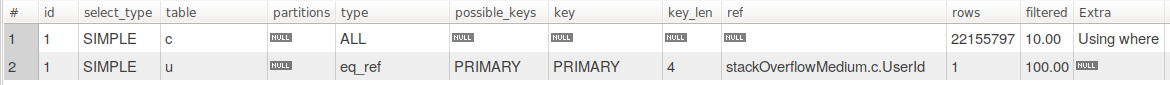
\includegraphics[scale =0.4]{explain7.png} 
	\caption{Przykład 1}
\end{figure}
\begin{spverbatim}
	EXPLAIN EXTENDED select p.Body from Posts p where p.Id = 875 union
	select c.`Text` from Comments c where c.PostID = 875;
\end{spverbatim}
\begin{figure}[h]
	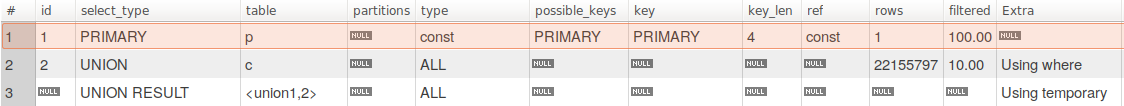
\includegraphics[scale =0.4]{explain8.png} 
	\caption{Przykład 2}
\end{figure}
\begin{spverbatim}
	EXPLAIN EXTENDED select * from Comments where UserId = (select id from Users where DisplayName = 'Jarrod Dixon');
\end{spverbatim}
\begin{figure}[h]
	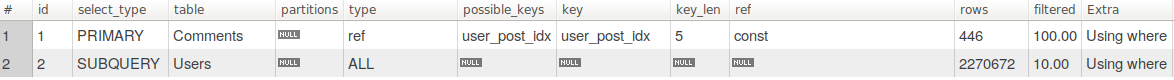
\includegraphics[scale =0.4]{explain9.png} 
	\caption{Przykład 3}
\end{figure}
\begin{spverbatim}
	EXPLAIN SELECT * FROM Comments where UserID in ( select UserId from Posts group by UserId having count(*) > 10);
\end{spverbatim}
\begin{figure}[h]
	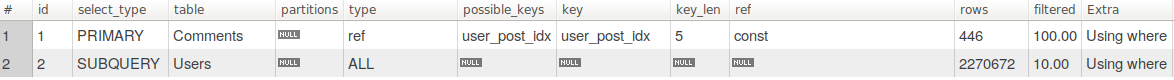
\includegraphics[scale =0.4]{explain9.png} 
	\caption{Przykład 4}
\end{figure}
\begin{figure}[h]
	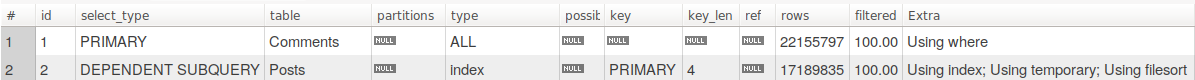
\includegraphics[scale =0.4]{explain10.png} 
	\caption{Przykład 5}
\end{figure}
\begin{figure}[h]
	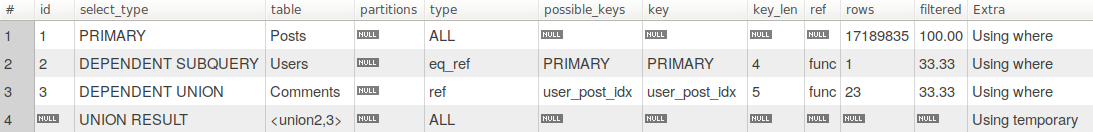
\includegraphics[scale =0.4]{explain11.png} 
	\caption{Przykład 6}
\end{figure}
\begin{figure}[h]
	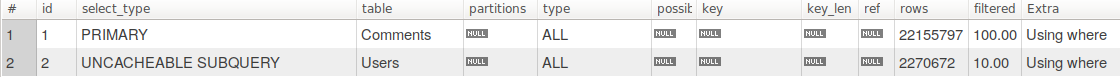
\includegraphics[scale =0.4]{explain12.png} 
	\caption{Przykład 7}
\end{figure}


\paragraph{Kolumna ID}\leavevmode\\
Kolumna id zawiera numer zapytania, którego dotyczy. W przypadku zapytań z podzapytaniami, podzapytania w dyrektywie FROM oraz zapytań z słowem kluczowym JOIN podzapytania numerowane są najczęściej względem ich występowania w zapytaniu. Kolumna ID może przyjąć również wartość NULL, w przypadku polecenia UNION (przykład 2).

\paragraph{Kolumna select\textunderscore type}\leavevmode\\
Kolumna select\textunderscore type pokazuje, czy rekord jest prostym, czy złożonym zapytaniem SELECT. 
Wartość \textbf{SIMPLE} oznacza, że zapytanie nie zawiera podzapytań, oraz nie używa klauzuli UNION.

Jeżeli natomiast zapytanie zawiera podzapytania lub wykorzystuje klauzulę UNION, to rekord dla kolumny select\textunderscore type przyjmie wartość \textbf{PRIMARY} (przykład 2). Jeżeli rekord dotyczy podzapytania oznaczonego jako PRIMARY, to będzie oznaczony jako \textbf{SUBQUERY} (przykład 3). Jako \textbf{UNION} zostaną oznaczone zapytania, które są drugim i kolejnym zapytaniem w klauzuli UNION. Pierwsze zapytanie zostanie oznaczone tak samo, jakby było wykonywane jako zwykłe zapytanie SELECT (przykład 2). \textbf{DERIVED} oznacza, że zapytanie jest umieszczone jako podzapytanie w klauzuli FROM, jest wykonywane rekurencyjnie i wyniki są umieszczane w tabeli tymczasowej. Wartość \textbf{UNION RESULT} oznacza wiersz, jako polecenie SELECT użyte do pobrania wyników z tabeli tymczasowej użytej przy poleceniu UNION (przykład 2). Jeśli polecenie SELECT zależy od danych znajdujących się w podzapytaniu lub znajdujących się w wyniki klazuli UNION, to zostanie oznaczone odpowiednio jako \textbf{DEPENDENT SUBQUERY} (przykład 5) lub \textbf{DEPENDENT UNION} (Przykład 6). Dodatkowo w przypadku, jeżeli wynik zwracany jest z \textit{zmaterializowanego widoku (eng. materialized view)}, zapytanie zostanie oznaczone jako \textbf{MATERIALIZED}. W przykładzie 7, który jest oczywiście nonsensowny, ale dobrze obrazuje sytuację, kiedy jako select\textunderscore type otrzymamy wartość \textbf{UNCACHABLE\textunderscore SUBQUERY}, która oznacza, że coś w podzapytaniu uniemożliwiło jego buforowanie. Analogiczną sytuację mamy, jeżeli wiersz zostanie oznaczony jako \textbf{UNCACHABLE\textunderscore UNION}, ale w tym przypadku niemożliwe jest oczywiście buforowanie wyników polecenia UNION.

\paragraph{Kolumna table}\leavevmode\\
Kolumna table w większości przypadków prezentuje nazwę tabeli lub jej alias, do której odnosi się dany wiersz wyniku polecenia \textit{EXPLAIN}. 